%!TEX root = ../main.tex
%%%%%%%%%%%%%%%%%%%%%%%%%%%%%%%%%%
% Links:
%
% Difficulty:
% Companies: 
%%%%%%%%%%%%%%%%%%%%%%%%%%%%%%%%%%


%\begin{figure}
%	\centering
%	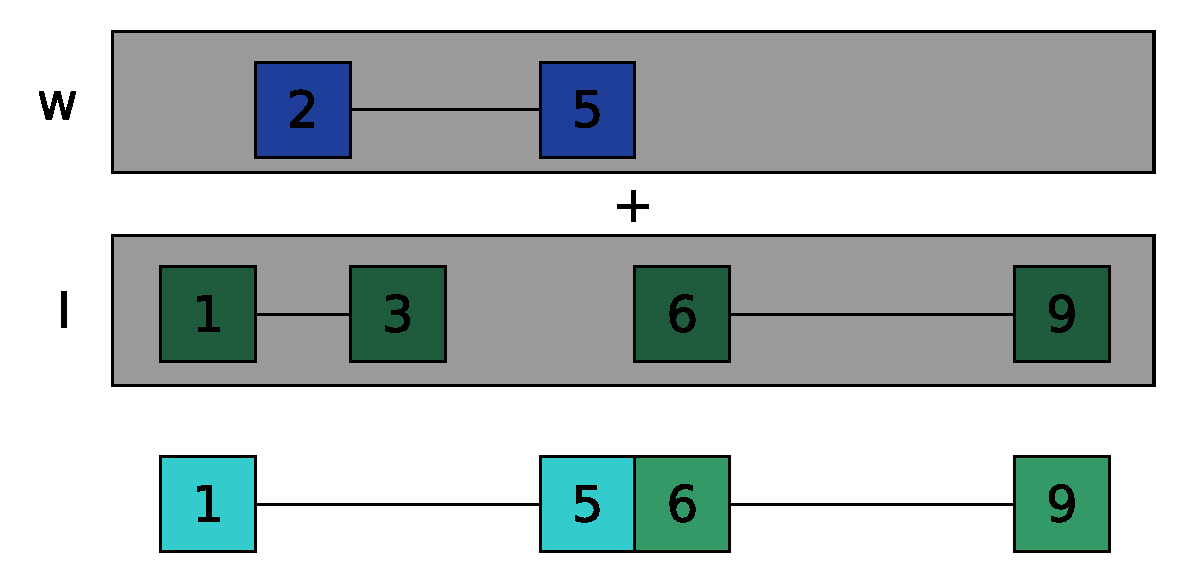
\includegraphics[width=\textwidth]{sources/merge_intervals_2/images/example1}
%	\caption[Sample short cpation]{Sample Caption}.
%	\label{fig:merge_intervals_2:example1}
%\end{figure}

\chapter{Merge Intervals}
\label{ch:merge_intervals_2}
\section*{Introduction}

\section{Problem statement}
\begin{exercise}
\label{example:merge_intervals_2:exercice1}
\begin{verbatim}
	
	Given a sorted list of disjoint (non-overlapping) intervals $I$ and an interval $w$
	insert $w$ into $I$ so that the 
	You may assume that the intervals were initially sorted according to their start times.
	
	Example 1:
	
	Given intervals [1,3],[6,9] insert and merge [2,5] would result in [1,5],[6,9].
	
	Example 2:
	
	Given [1,2],[3,5],[6,7],[8,10],[12,16], insert and merge [4,9] would result in [1,2],[3,10],[12,16].
	
	This is because the new interval [4,9] overlaps with [3,5],[6,7],[8,10].
	
	Make sure the returned intervals are also sorted.
\end{verbatim}

	%example1
	\begin{example}
		\label{example:merge_intervals_2:example1}
		\hfill \\
	
		
	\end{example}

	%example2
	\begin{example}
		\label{example:merge_intervals_2:example2}
		\hfill \\
		
	\end{example}

	\begin{example}
		\hfill \\
	
	\label{ex:merge_intervals_2:example3}
	\end{example}

	\begin{example}
		\hfill \\

	\label{ex:merge_intervals_2:example4}	
	\end{example}
\end{exercise}

\section{Clarification Questions}

\begin{QandA}
	\item 
	\begin{answered}
		\textit{}
	\end{answered}
	
\end{QandA}

\section{Discussion}
\label{merge_intervals_2:sec:discussion}


\subsection{Brute-force}
\label{merge_intervals_2:sec:bruteforce}

\begin{minipage}{\linewidth}
	\lstinputlisting[language=c++, caption={Sample Caption},label=list:merge_intervals_2]{sources/merge_intervals_2/merge_intervals_2_solution1.cpp}
\end{minipage}

